% Provenance (never printed): cycle 4 SVT, "La planete Terre, l'environnement
% et l'action humaine": climate, its past variations and the present change,
% read from data; see sources/book1/PROVENANCE.md. Book 1, grade 9, chapter 1.
% Vocabulary guard: owns climate change (first look; Book 2 g12 re-uses it),
% global warming, temperature anomaly. The greenhouse effect and greenhouse
% gases belong to the chemistry series (grade 8): recalled in prose, never
% defined. Infrared is physics (g10): named in prose only. "Glacial period"
% and "interglacial" belong to Book 2 g12: here "the ice ages and the warmer
% times between them". Physical science only, in the IPCC's calibrated words;
% no policy.
\chapter{O clima da Terra, passado e presente}\label{ch:g9:climate-past-and-present}

Se a Terra não tivesse ar em volta, mas refletisse a mesma parte da luz
do Sol que reflete hoje, a sua superfície ficaria a uma temperatura média
de cerca de \qty{-19}{\degreeCelsius}: \omterm{def:g2:water-on-earth:ocean}{mares} congelados, terras
congeladas, em toda parte. A sua média real é de cerca de
\qty{15}{\degreeCelsius}. A diferença, uns \qty{34}{\degreeCelsius}, vem
de alguns gases do ar, presentes em quantidades minúsculas, que impedem
parte do calor da Terra de escapar para o espaço. Este capítulo trata
desses gases, do \omterm{def:g5:weather-and-climate:climate}{clima} da Terra no passado e de como e por que ele está
mudando agora.
% ledger: earth:Tbb, earth:Tsurf (figdata/grade-9/climate_records.py: -19.1 and 14.9 degC, gap 34)

\begin{recall}
O \omterm{def:g5:weather-and-climate:climate}{clima} de um lugar é o \omterm{def:g1:watching-the-weather:weather}{tempo} que ele costuma ter, em média ao longo de
30 anos (\cref{ch:g5:weather-and-climate}). A camada mais baixa da
atmosfera, onde o \omterm{def:g1:watching-the-weather:weather}{tempo} acontece, é a \omterm{def:g8:the-atmosphere:layers}{troposfera}
(\cref{ch:g8:the-atmosphere}). As \omterm{def:g8:ice-on-earth:ice-age}{glaciações}, com \omterm{def:g8:ice-on-earth:ice-sheet}{mantos de gelo} muito
além dos \omterm{def:g3:continents-and-oceans:poles}{polos}, vieram e se foram; o \omterm{def:g8:ice-on-earth:sea-ice}{gelo marinho} do Ártico encolheu
desde 1979 (\cref{ch:g8:ice-on-earth}). Em química, você aprende que o
gás carbônico, o metano e o vapor de água são \emph{gases de efeito
estufa}: eles deixam passar a luz do Sol, mas absorvem a luz
infravermelha invisível emitida pelo chão aquecido, o que é o
\emph{efeito estufa}; queimar carvão, petróleo e gás libera gás carbônico.
\end{recall}

\section{O efeito estufa e a temperatura da Terra}

A luz do Sol atravessa a atmosfera e aquece o chão e os \omterm{def:g2:water-on-earth:ocean}{oceanos}. Como
todo corpo quente, a superfície aquecida emite energia por sua vez, na
forma de luz infravermelha, que o olho não vê. Se toda ela escapasse para
o espaço, a Terra seria o mundo congelado do primeiro parágrafo. Mas os
gases de efeito estufa do ar absorvem grande parte dessa luz
infravermelha e mandam parte dela de volta para baixo: a superfície
recebe energia ao mesmo tempo do Sol e do ar acima dela, e se estabiliza
numa temperatura mais alta.

\begin{omfigure}
\begin{tikzpicture}[font=\footnotesize, >={Stealth[length=2.4mm]}]
  % ground and atmosphere
  \fill[omLithAlluv] (0,0) rectangle (12,0.5);
  \fill[omSea!45] (0,0.5) rectangle (12,3.4);
  \node[anchor=north east, align=right] at (11.85,3.35) {atmosfera com gases\\ de efeito estufa};
  \node[anchor=south east] at (11.9,0.05) {chão e oceanos};
  \node[anchor=south west] at (0.15,3.5) {espaço};
  % Sun
  \fill[omWxSun] (1.3,5.0) circle (0.45);
  \node at (1.3,4.3) {Sol};
  % sunlight in
  \draw[->, omWxSun!80!black, line width=2.2pt] (1.7,4.6) -- (2.7,0.55)
    node[pos=0.25, right=2pt, align=left, black] {a luz do Sol entra\\ e aquece a superfície};
  % infrared out and back
  \draw[->, omWarm, line width=1.6pt, decorate, decoration={snake, amplitude=1mm, segment length=4mm, post length=3mm}]
    (6.0,0.55) -- (6.6,2.6);
  \draw[->, omWarm, line width=1.6pt, decorate, decoration={snake, amplitude=1mm, segment length=4mm, post length=3mm}]
    (6.6,2.7) -- (7.4,5.0) node[right, align=left, black] {uma parte escapa\\ para o espaço};
  \draw[->, omWarm, line width=1.6pt, decorate, decoration={snake, amplitude=1mm, segment length=4mm, post length=3mm}]
    (6.8,2.75) -- (8.6,0.55);
  \node[align=left, anchor=west] at (8.8,1.9) {parte é absorvida\\ pelos gases e\\ devolvida};
  \node[align=right, anchor=east] at (5.9,1.3) {a superfície aquecida\\ emite infravermelho};
\end{tikzpicture}

{\small O efeito estufa, de forma simples (um esboço). Sem ele, a
superfície da Terra teria em média cerca de \qty{-19}{\degreeCelsius};
com ele, cerca de \qty{15}{\degreeCelsius}.}
% ledger: earth:Tbb, earth:Tsurf
\label{fig:g9:climate-past-and-present:greenhouse}
\end{omfigure}

O efeito estufa é natural e necessário: sem ele, não haveria água líquida
na superfície. A pergunta deste capítulo é outra: o que acontece com a
temperatura da Terra quando a quantidade de gases de efeito estufa no ar
muda?

\section{Os climas do passado}

Para ler o \omterm{def:g5:weather-and-climate:climate}{clima} do passado distante, os cientistas perfuram os \omterm{def:g8:ice-on-earth:ice-sheet}{mantos
de gelo}. Todo ano, cai \omterm{def:g4:clouds-rain-snow:precipitation}{neve} sobre a Antártida e a Groenlândia, e a \omterm{def:g4:clouds-rain-snow:precipitation}{neve}
do verão é um pouco diferente da \omterm{def:g4:clouds-rain-snow:precipitation}{neve} do inverno. Enterradas e
comprimidas em gelo, as camadas anuais permanecem, uma acima da outra,
como as páginas de um livro. Quanto mais fundo o gelo, mais antigo ele é.
% ledger: eo:ice-core

\begin{omfigure}
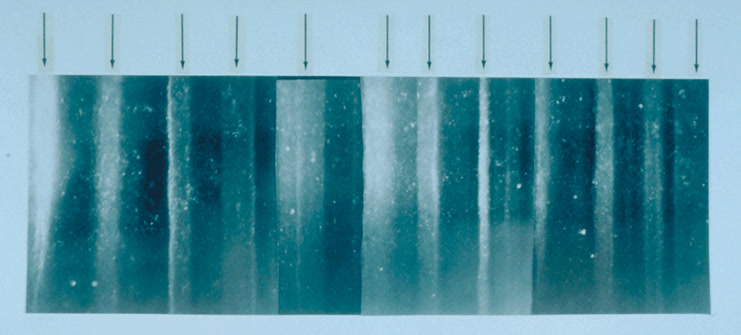
\includegraphics[width=0.78\linewidth]{images/book1/g9-gisp2-layers.jpg}

{\small Um trecho de testemunho de gelo de \qty{19}{cm} de comprimento,
perfurado a uma profundidade de \qty{1855}{m} no \omterm{def:g8:ice-on-earth:ice-sheet}{manto de gelo} da
Groenlândia e iluminado por baixo. As setas apontam as camadas de verão,
mais claras, entre camadas de inverno mais escuras: onze anos de \omterm{def:g4:clouds-rain-snow:precipitation}{neve}.
NOAA Paleoclimatology (domínio público, via Wikimedia Commons).}
% ledger: commons:gisp2-layers
\label{fig:g9:climate-past-and-present:ice-core}
\end{omfigure}

Um testemunho de gelo guarda dois registros do passado. A própria \omterm{def:g4:clouds-rain-snow:precipitation}{neve}
diz quão frio estava o ar quando ela caiu: quanto mais frio o ar, menor a
parte das formas mais pesadas de hidrogênio e de oxigênio na \omterm{def:g4:clouds-rain-snow:precipitation}{neve}. E,
quando a \omterm{def:g4:clouds-rain-snow:precipitation}{neve} é comprimida em gelo, os espaços entre os grãos se fecham,
prendendo bolhas minúsculas do ar da época. Os cientistas liberam esse ar
antigo no laboratório e medem o seu gás carbônico.
% ledger: eo:ice-core

\begin{omfigure}
\begin{tikzpicture}
\begin{axis}[name=temp, omrecord, omage, width=13cm, height=3.9cm, xmin=0, xmax=800,
  xtick={0,100,...,800}, xticklabels={}, ylabel={variação de\\ temperatura ($^\circ$C)},
  ylabel style={align=center}, ymin=-11, ymax=5, ytick={-10,-5,0,5}]
  \addplot[omWarm, line width=0.7pt] table[x=age_kyr, y=temp_C] {figdata/out/grade-9-climate_records-edc.dat};
\end{axis}
\begin{axis}[at={(temp.south west)}, anchor=north west, yshift=-0.3cm, omrecord, omage,
  width=13cm, height=3.9cm, xmin=0, xmax=800, xtick={0,100,...,800},
  xlabel={milhares de anos antes de hoje}, ylabel={gás carbônico\\ (ppm)},
  ylabel style={align=center}, ymin=160, ymax=320, ytick={180,220,260,300}]
  \addplot[black, line width=0.7pt] table[x=age_kyr, y=co2_ppm] {figdata/out/grade-9-climate_records-icecore.dat};
\end{axis}
\end{tikzpicture}

{\small Oitocentos mil anos lidos no gelo da Antártida. Em cima: a
variação da temperatura do ar em Dome~C, comparada com a média dos
últimos mil anos (testemunho de gelo EPICA Dome~C, J.~Jouzel e
colaboradores, 2007). Embaixo: o gás carbônico do ar preso no gelo, em
partes por milhão (B.~Bereiter e colaboradores, 2015). Ambos em médias
por intervalos de \num{2000} anos; o tempo corre da esquerda (mais
antigo) para a direita (hoje).}
% ledger: data:edc-jouzel, data:co2-bereiter (figdata/grade-9/climate_records.py)
\label{fig:g9:climate-past-and-present:icecore}
\end{omfigure}

As duas curvas contam a mesma história. Repetidas vezes, longos períodos
frios, as \omterm{def:g8:ice-on-earth:ice-age}{glaciações}, deram lugar a períodos quentes mais curtos, e depois
o frio voltou. No auge do frio, o ar sobre a Antártida estava cerca de
\qty{9}{\degreeCelsius} mais frio do que nos últimos mil anos; nos
períodos mais quentes, estava alguns graus mais quente. E o gás carbônico
subiu e desceu junto com a temperatura, entre cerca de \qty{175}{ppm} nos
períodos frios e cerca de \qty{300}{ppm} nos quentes. Vivemos num dos
períodos quentes, que começou quando a última \omterm{def:g8:ice-on-earth:ice-age}{glaciação} terminou.
% ledger: data:edc-jouzel, data:co2-bereiter (figdata/grade-9/climate_records.py: edc min -9.7, max +3.6; CO2 174 to 299 ppm)

\begin{method}[Ler dois registros lado a lado]
\begin{enumerate}
  \item Verifique se os dois registros têm o mesmo eixo do tempo, e em
        que sentido o tempo corre.
  \item Escolha uma data no eixo do tempo e leia cada registro nessa data.
  \item Procure os picos e os \omterm{def:g1:landscapes-around-us:landform}{vales}: eles aparecem nas mesmas épocas nos
        dois registros?
  \item Diga o que varia junto, sem decidir ainda qual mudança causou
        a outra.
\end{enumerate}
\end{method}

\begin{example}[A última glaciação no testemunho de gelo]
Há \num{20000} anos (o 20 do eixo do tempo), a curva da temperatura está
em cerca de \qty{-9}{\degreeCelsius} e o gás carbônico em cerca de
\qty{190}{ppm}. Nos últimos mil anos, a curva da temperatura está perto
de 0 e o gás carbônico perto de \qty{280}{ppm}. Então, no auge do frio
da última \omterm{def:g8:ice-on-earth:ice-age}{glaciação}, o ar sobre a Antártida estava cerca de
\qty{9}{\degreeCelsius} mais frio, e continha cerca de
$280 - 190 = \qty{90}{ppm}$ a menos de gás carbônico, um terço a menos.
\end{example}
% ledger: data:edc-jouzel, data:co2-bereiter (figdata/grade-9/climate_records.py: 19-21 kyr bins -9.4, 190 ppm; 1 kyr bin 278)

Mais para trás ainda, a Terra conheceu \omterm{def:g5:weather-and-climate:climate}{climas} muito mais quentes do que
qualquer um dos últimos 800\,000 anos. As avaliações científicas estimam
que a última vez em que a superfície da Terra ficou
\qty{2.5}{\degreeCelsius} ou mais acima do seu nível do fim do século~XIX
foi há mais de três milhões de anos.
% ledger: ipcc:3myr

\section{Os registros de hoje}

Desde o fim do século~XIX, a temperatura é medida todos os dias em
milhares de \omterm{def:g4:clouds-rain-snow:weather-station}{estações meteorológicas} em terra e no \omterm{def:g2:water-on-earth:ocean}{mar}, com termômetros
mantidos à sombra. Para acompanhar o planeta inteiro, os cientistas não
fazem a média das próprias temperaturas, que dependem de onde fica cada
estação, mas do quanto cada uma se afasta do seu próprio valor habitual.
% ledger: giss:method

\begin{definition}[Anomalia de temperatura]\label{def:g9:climate-past-and-present:anomaly}
Uma \emph{anomalia de temperatura}\index{anomalia de temperatura} é a
diferença entre uma temperatura e a sua média ao longo de um período de
referência escolhido. Ela é positiva quando está mais quente do que essa
média, negativa quando está mais frio.
\end{definition}

\begin{omfigure}
\begin{minipage}[c]{0.44\linewidth}\centering
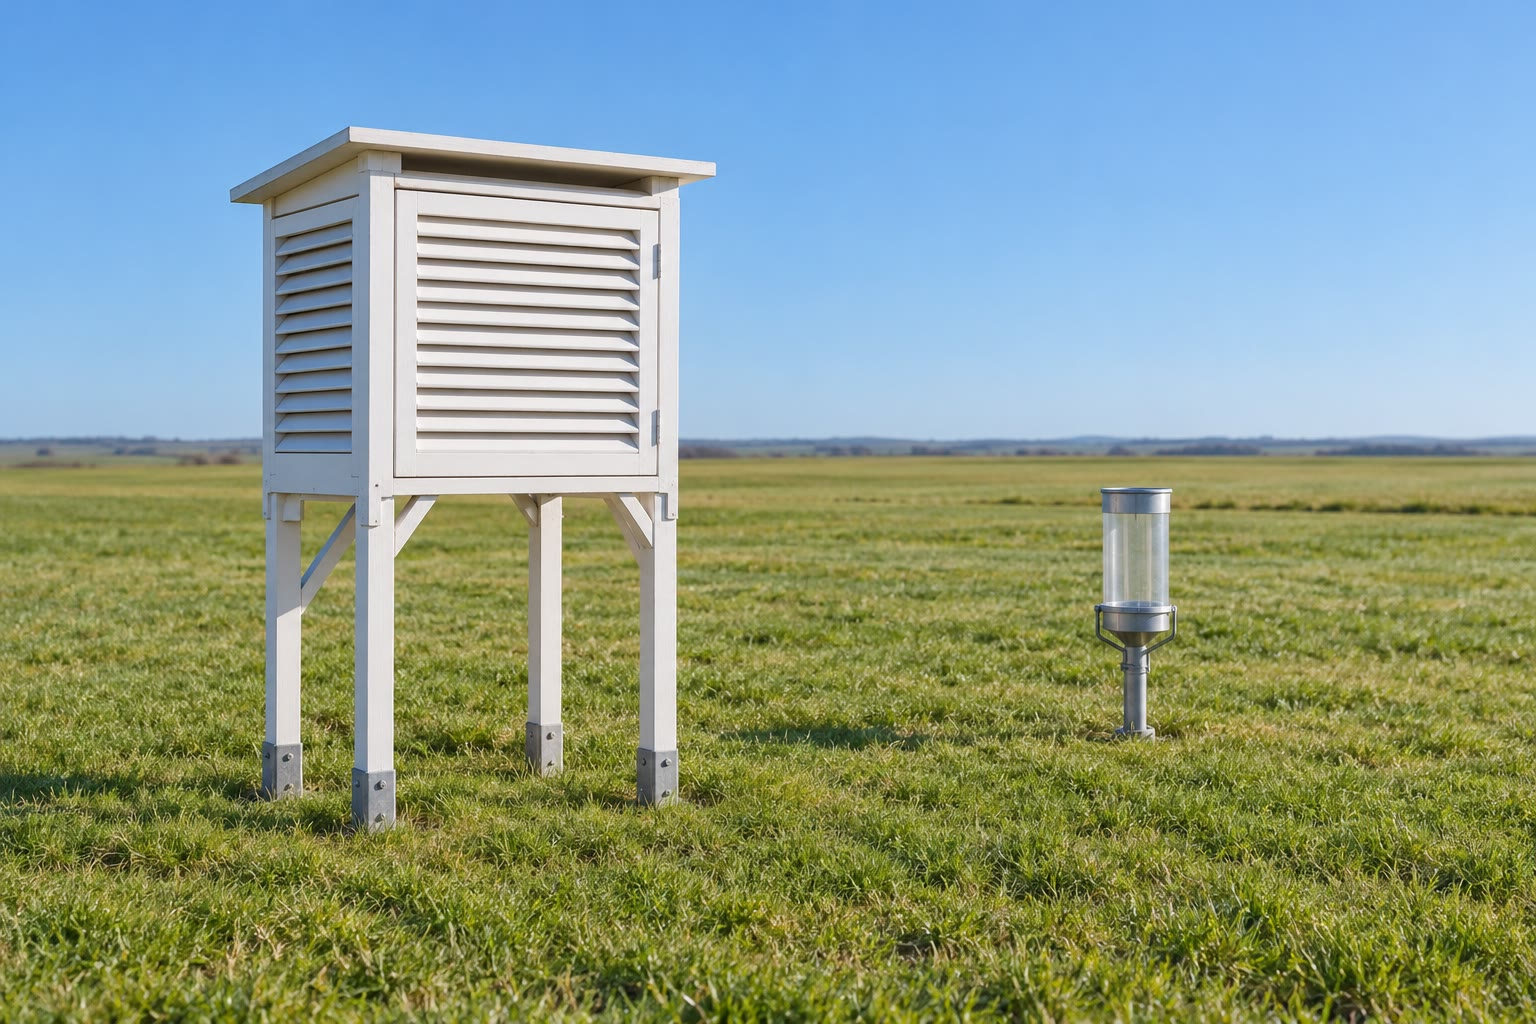
\includegraphics[width=\linewidth]{images/book1/ai/g9-weather-screen.jpg}
\end{minipage}\hfill
\begin{minipage}[c]{0.52\linewidth}\raggedright
{\small Uma \omterm{def:g4:clouds-rain-snow:weather-station}{estação meteorológica}: a caixa branca sobre pés, com laterais
em venezianas, mantém os termômetros à sombra enquanto o ar passa por
ela; à direita, um \omterm{def:g4:clouds-rain-snow:rain-gauge}{pluviômetro} (ilustração gerada por IA de uma cena
genérica).}
\end{minipage}
\label{fig:g9:climate-past-and-present:screen}
\end{omfigure}

O registro da temperatura global da NASA, por exemplo, dá a anomalia de
cada ano em relação à média de 1951--1980, a partir de estações em terra
e de medidas da superfície do \omterm{def:g2:water-on-earth:ocean}{mar}. Em médias década por década, ele
mostra uma subida clara.
% ledger: giss:method, data:gistemp

\begin{omfigure}
\begin{tikzpicture}
\begin{axis}[omrecord, ybar, width=13cm, height=5.6cm, bar width=9pt,
  ymin=-0.45, ymax=1.2, ytick={-0.4,0,0.4,0.8,1.2},
  xtick=data, xticklabels={anos 1880, anos 1890, anos 1900, anos 1910, anos 1920, anos 1930, anos 1940, anos 1950, anos 1960, anos 1970, anos 1980, anos 1990, anos 2000, anos 2010, 2020--25},
  x tick label style={rotate=60, anchor=east, font=\scriptsize},
  ylabel={anomalia de temperatura ($^\circ$C)}, xmajorgrids=false]
  \addplot[fill=omWarm!70, draw=black!50] table[x expr=\coordindex, y=mean_C]
    {figdata/out/grade-9-climate_records-decades.dat};
\end{axis}
\end{tikzpicture}

{\small A temperatura global da superfície, década por década desde os
anos 1880, como anomalia em relação à média de 1951--1980; a última barra
cobre os seis anos 2020--2025. Dados: NASA GISTEMP versão~4.}
% ledger: data:gistemp (figdata/grade-9/climate_records.py)
\label{fig:g9:climate-past-and-present:decades}
\end{omfigure}

\begin{definition}[Aquecimento global]\label{def:g9:climate-past-and-present:global-warming}
O \emph{aquecimento global}\index{aquecimento global} é a subida da
temperatura média da superfície da Terra, como um todo, desde a segunda
metade do século~XIX.
\end{definition}

Ano a ano, o registro sobe e desce: um ano pode ser mais fresco do que o
anterior, porque o \omterm{def:g1:watching-the-weather:weather}{tempo} de um ano inteiro, sobre \omterm{def:g2:water-on-earth:ocean}{oceanos} e \omterm{def:g3:continents-and-oceans:continent}{continentes},
também varia. Para medir um aquecimento, os cientistas comparam, por
isso, médias de muitos anos, nunca dois anos isolados.

\begin{omfigure}
\begin{tikzpicture}
\begin{axis}[omrecord, width=13cm, height=5.4cm, xmin=1875, xmax=2030, ymin=-0.6, ymax=1.4,
  xtick={1880,1900,...,2020}, x tick label style={/pgf/number format/1000 sep={}},
  xlabel={ano}, ylabel={anomalia de temperatura ($^\circ$C)},
  legend style={at={(0.2,0.97)}, anchor=north west, draw=none, fill=white, font=\footnotesize}]
  \fill[omWarm!10] (axis cs:1880,-0.6) rectangle (axis cs:1899,1.4);
  \fill[omWarm!10] (axis cs:2015,-0.6) rectangle (axis cs:2024,1.4);
  \addplot[black!70, mark=*, mark size=0.9pt, line width=0.4pt]
    table[x=year, y=anomaly_C] {figdata/out/grade-9-climate_records-annual.dat};
  \addlegendentry{cada ano}
  \addplot[omWarm, line width=2pt] table[x=year, y=mean_C] {figdata/out/grade-9-climate_records-periods.dat};
  \addlegendentry{média de um período}
  \draw[dashed, black!50] (axis cs:1875,0) -- (axis cs:2030,0);
  \node[font=\scriptsize, fill=white, inner sep=1pt] at (axis cs:1889.5,0.45) {1880--1899};
  \node[font=\scriptsize, fill=white, inner sep=1pt] at (axis cs:2019.5,0.3) {2015--2024};
\end{axis}
\end{tikzpicture}

{\small A anomalia da temperatura global de cada ano de 1880 a 2025 (em
relação à média de 1951--1980, linha tracejada), com as médias de dois
períodos do problema deste capítulo: 1880--1899 e 2015--2024. Dados:
NASA GISTEMP versão~4.}
% ledger: data:gistemp (figdata/grade-9/climate_records.py)
\label{fig:g9:climate-past-and-present:annual}
\end{omfigure}

\begin{method}[Medir um aquecimento entre dois períodos]
\begin{enumerate}
  \item Escolha dois períodos de pelo menos dez anos cada, um antigo e um
        recente, para que os altos e baixos de cada ano se compensem.
  \item Faça a média das anomalias anuais de cada período.
  \item Subtraia a média antiga da recente: o resultado é o aquecimento
        entre os dois períodos, em graus.
  \item Diga qual registro e quais períodos você usou: outro registro, ou
        outros períodos, dão um número um pouco diferente.
\end{enumerate}
\end{method}

\begin{example}[O aquecimento desde os anos 1970]
No registro da NASA, as anomalias dos dez anos 1970--1979 têm média de
\qty{0.03}{\degreeCelsius}, e as de 2010--2019, média de
\qty{0.80}{\degreeCelsius}. O aquecimento entre essas duas décadas é
$0.80 - 0.03 = \qty{0.77}{\degreeCelsius}$, em quarenta anos: cerca de
\qty{0.19}{\degreeCelsius} por década. Anos isolados, também com quarenta
anos de distância, dariam respostas muito diferentes: 1976 ($-0.10$)
contra 2016 (1.01) dá \qty{1.11}{\degreeCelsius}, mas 1979 (0.16) contra
2011 (0.61) dá só \qty{0.45}{\degreeCelsius}.
\end{example}
% ledger: data:gistemp (figdata/grade-9/climate_records.py: decade_1970s 0.03, decade_2010s 0.80; annual 1976 -0.10, 2016 1.01, 1979 0.16, 2011 0.61)

O gás carbônico do ar é medido diretamente desde março de 1958, num
observatório a cerca de \qty{3400}{m} de \omterm{def:g4:world-physical-map:altitude}{altitude}, nas encostas do \omterm{def:g4:volcanoes-earthquakes-first-look:volcano}{vulcão}
Mauna Loa, no Havaí. Em 1959, a sua média anual era de \qty{316}{ppm};
em 2025, tinha chegado a \qty{427}{ppm}, muito acima dos \qty{300}{ppm}
que ele nunca ultrapassou em 800\,000 anos de gelo. Ele sobe cada vez
mais depressa: menos de \qty{1}{ppm} por ano nos anos 1960, mais de
\qty{2.5}{ppm} por ano nos últimos dez anos.
% ledger: gml:keeling, data:co2-mlo, data:co2-bereiter (figdata/grade-9/climate_records.py: 315.98, 427.35, 0.86 and 2.63 ppm/yr; ice core max 298.6)

\begin{omfigure}
\begin{tikzpicture}
\begin{axis}[omrecord, width=12cm, height=5cm, xmin=1955, xmax=2030,
  ymin=290, ymax=440, ytick={300,350,400}, xtick={1960,1970,...,2020},
  x tick label style={/pgf/number format/1000 sep={}},
  xlabel={ano}, ylabel={gás carbônico (ppm)}]
  \addplot[black, line width=0.9pt, mark=*, mark size=0.8pt] table[x=year, y=co2_ppm] {figdata/out/grade-9-climate_records-co2.dat};
  \draw[dashed, omWarm] (axis cs:1955,300) -- (axis cs:2030,300);
\end{axis}
\end{tikzpicture}

{\small O gás carbônico do ar em Mauna Loa, no Havaí, médias anuais
1959--2025 (NOAA Global Monitoring Laboratory e Scripps Institution of
Oceanography). A linha tracejada em \qty{300}{ppm} é mais ou menos o
nível mais alto encontrado em 800\,000 anos de gelo da Antártida.}
% ledger: data:co2-mlo, data:co2-bereiter (figdata/grade-9/climate_records.py)
\label{fig:g9:climate-past-and-present:co2}
\end{omfigure}

\begin{dated}{2025}
A média anual do gás carbônico em Mauna Loa foi de \qty{427.35}{ppm} em
2025. No registro da NASA, o ano mais quente desde 1880 foi 2024, com uma
anomalia de \qty{1.28}{\degreeCelsius} em relação a 1951--1980.
% ledger: data:co2-mlo, data:gistemp (figdata/grade-9/climate_records.py)
\end{dated}

O \omterm{def:g2:water-on-earth:ocean}{mar} também está subindo. Desde 1993, satélites medem a altura da
superfície do \omterm{def:g2:water-on-earth:ocean}{mar} no \omterm{def:g3:continents-and-oceans:globe}{globo} inteiro: a linha de tendência do seu registro
sobe cerca de \qty{3.2}{mm} por ano, cerca de \qty{10}{cm} em trinta
anos. Duas coisas fazem o \omterm{def:g2:water-on-earth:ocean}{mar} subir: a água que se aquece se expande, e o
gelo que derrete em terra acrescenta água ao \omterm{def:g2:water-on-earth:ocean}{oceano}. E o gelo está
encolhendo: as \omterm{def:g8:ice-on-earth:glacier}{geleiras} de \omterm{def:g1:landscapes-around-us:landform}{montanha} recuam em quase toda parte, e o \omterm{def:g8:ice-on-earth:sea-ice}{gelo
marinho} de verão do Ártico perdeu quase metade da sua extensão desde 1979
(\cref{ch:g8:ice-on-earth}).
% ledger: data:gmsl-lsa (figdata/grade-9/climate_records.py: 3.18 mm/yr; 101 mm 1993-2024), ipcc:b1-ice, nsidc:ice-shelves, data:b1-nsidc-sea-ice

\begin{omfigure}
\begin{tikzpicture}
\begin{axis}[omrecord, width=12cm, height=4.8cm, xmin=1992, xmax=2026,
  ymin=-30, ymax=100, xtick={1995,2000,...,2025},
  x tick label style={/pgf/number format/1000 sep={}},
  xlabel={ano}, ylabel={nível do mar (mm)},
  legend style={at={(0.02,0.97)}, anchor=north west, draw=none, fill=white, font=\footnotesize}]
  \addplot[omCold, mark=*, mark size=1.1pt, line width=0.6pt] table[x=year, y=gmsl_mm] {figdata/out/grade-9-climate_records-sea.dat};
  \addlegendentry{média anual}
  \addplot[omWarm, dashed, line width=0.9pt] table[x=year, y=gmsl_mm] {figdata/out/grade-9-climate_records-sea-trend.dat};
  \addlegendentry{linha de tendência}
\end{axis}
\end{tikzpicture}

{\small O nível médio global do \omterm{def:g2:water-on-earth:ocean}{mar} medido por satélites, médias anuais
1993--2024, em relação a um nível de referência, e a sua linha de
tendência (NOAA Laboratory for Satellite Altimetry).}
% ledger: data:gmsl-lsa (figdata/grade-9/climate_records.py)
\label{fig:g9:climate-past-and-present:sea}
\end{omfigure}

\section{A mudança climática e as suas causas}

\begin{definition}[Mudança climática]\label{def:g9:climate-past-and-present:climate-change}
Uma \emph{mudança climática}\index{mudanca climatica@mudança climática} é uma mudança do
\omterm{def:g5:weather-and-climate:climate}{clima} da Terra, ou de uma região, que dura décadas ou mais: uma mudança da
sua temperatura média, das \omterm{def:g4:clouds-rain-snow:precipitation}{chuvas}, dos ventos ou do gelo, e não apenas
uma estação fora do comum.
\end{definition}

O \omterm{def:g5:weather-and-climate:climate}{clima} sempre mudou, como mostram os testemunhos de gelo. O que é novo é
a velocidade da mudança de hoje, e a sua causa. Cientistas do mundo
inteiro avaliam regularmente o que foi publicado sobre o \omterm{def:g5:weather-and-climate:climate}{clima}, nos
relatórios do Painel Intergovernamental sobre Mudanças Climáticas (IPCC).
Os relatórios pesam quão certa é cada afirmação, com palavras escolhidas
com cuidado.

Nesses relatórios, cada uma das expressões abaixo tem um sentido fixo: as
chances em 100 de que a afirmação seja verdadeira.

\begin{center}
{\small
\begin{tabular}{|l|c||l|c|}
\hline
\emph{virtualmente certo} & 99 a 100 & \emph{provável} & 66 a 100 \\
\emph{extremamente provável} & 95 a 100 & \emph{tão provável quanto não} & 33 a 66 \\
\emph{muito provável} & 90 a 100 & \emph{improvável} & 0 a 33 \\
\hline
\end{tabular}}
\end{center}
% ledger: ipcc:likelihood

\noindent Algumas afirmações não trazem nenhuma dessas expressões: elas
são dadas como fatos, como ``é \emph{inequívoco}''. Quando você ler uma
notícia sobre o \omterm{def:g5:weather-and-climate:climate}{clima}, procure essas expressões e repare quais a notícia
mantém e quais ela deixa de lado.
% ledger: ipcc:unequivocal

A avaliação publicada em 2021 afirma o seguinte.
\begin{itemize}
  \item É \emph{inequívoco} que a influência humana aqueceu a atmosfera,
        o \omterm{def:g2:water-on-earth:ocean}{oceano} e as terras.
  \item A temperatura global da superfície de 2011--2020 foi cerca de
        \qty{1.1}{\degreeCelsius} mais alta do que em 1850--1900, e cada
        uma das últimas quatro décadas foi mais quente do que qualquer
        década anterior desde 1850.
  \item O aquecimento causado pelo ser humano de 1850--1900 a 2010--2019
        é \emph{provavelmente} de 0.8 a \qty{1.3}{\degreeCelsius}, com
        uma melhor estimativa de \qty{1.07}{\degreeCelsius}: praticamente
        todo o aquecimento observado. As causas naturais, juntas,
        mudaram a temperatura em apenas $-0.1$ a $+\qty{0.1}{\degreeCelsius}$.
  \item O gás carbônico do ar em 2019 era mais alto do que em qualquer
        momento de pelo menos dois milhões de anos (\emph{alta
        confiança}); ele tinha subido 47~\% desde 1750.
  \item A influência humana é \emph{muito provavelmente} a principal
        causa do recuo das \omterm{def:g8:ice-on-earth:glacier}{geleiras} desde os anos 1990 e do encolhimento
        do \omterm{def:g8:ice-on-earth:sea-ice}{gelo marinho} do Ártico; e \emph{muito provavelmente} a
        principal causa da subida do \omterm{def:g2:water-on-earth:ocean}{mar} desde pelo menos 1971.
\end{itemize}
% ledger: ipcc:unequivocal, ipcc:gsat-2011-2020, ipcc:decades, ipcc:attribution, ipcc:co2-2myr, ipcc:b1-ice, ipcc:sea-level-obs

\begin{history}[A curva de Charles David Keeling]
Em março de 1958, um jovem químico da Scripps Institution of
Oceanography, Charles David Keeling, começou a medir o gás carbônico do
ar no Mauna Loa, bem acima do \omterm{def:g2:water-on-earth:ocean}{mar} e longe de qualquer cidade. As suas
medidas continuam desde então: são o registro mais longo de gás carbônico
medido diretamente no ar, e a curva que elas desenham, subindo ano após
ano, leva o seu nome, a \emph{curva de Keeling}.
% ledger: gml:keeling
\end{history}

Por que o aquecimento acompanha o gás carbônico? Queimar carvão, petróleo
e gás libera gás carbônico; mais gás carbônico no ar quer dizer que mais
da luz infravermelha emitida pela superfície é absorvida e mandada de
volta para baixo, e a superfície se aquece. O vapor de água, o metano e os
outros gases de efeito estufa somam-se ao efeito. O passado e o presente
concordam: nos testemunhos de gelo como nos registros de hoje, a
temperatura da Terra e o seu gás carbônico sobem e descem juntos.
% ledger: ipcc:attribution, ipcc:co2-2myr

\section{Exercícios}

\begin{exercise}[$\star$]\label{exo:g9:climate-past-and-present:1}
% ledger: earth:Tbb, earth:Tsurf
(a) Qual seria a temperatura média da superfície da Terra sem o efeito
estufa? (b) Qual é ela com o efeito estufa? (c) Em quantos graus o efeito
estufa aquece a superfície? (d) Cite dois gases de efeito estufa.
\end{exercise}

\begin{exercise}[$\star$]\label{exo:g9:climate-past-and-present:2}
\omterm{def:g1:watching-the-weather:weather}{Tempo} ou \omterm{def:g5:weather-and-climate:climate}{clima}? (a) Choveu o dia inteiro ontem. (b) Os verões desta
região são quentes e secos. (c) Os anos 2010 foram mais quentes do que os
anos 1980 no mundo todo. (d) A semana que vem vai ser fria.
\end{exercise}

\begin{exercise}[$\star$]\label{exo:g9:climate-past-and-present:3}
% ledger: commons:gisp2-layers
Observe a fotografia do trecho de testemunho de gelo. (a) Qual é o
comprimento do trecho, e quantos anos de \omterm{def:g4:clouds-rain-snow:precipitation}{neve} ele contém? (b) Encontre a
espessura média da camada de um ano, em centímetros. (c) Por que o gelo
mais profundo de um \omterm{def:g8:ice-on-earth:ice-sheet}{manto de gelo} é o mais antigo?
\end{exercise}

\begin{exercise}[$\star$]\label{exo:g9:climate-past-and-present:4}
A temperatura média de julho de uma cidade em 1991--2020 é de
\qty{21.0}{\degreeCelsius}. Dê a \omterm{def:g9:climate-past-and-present:anomaly}{anomalia de temperatura} de um mês de
julho com média de (a) \qty{22.4}{\degreeCelsius}; (b)
\qty{20.3}{\degreeCelsius}; (c) \qty{21.0}{\degreeCelsius}. (d) O que
quer dizer uma anomalia negativa?
\end{exercise}

\begin{exercise}[$\star\star$]\label{exo:g9:climate-past-and-present:5}
% ledger: data:gistemp (figdata/grade-9/climate_records.py)
Use o gráfico de barras das décadas. (a) Quais décadas foram mais frias
do que a média de 1951--1980? (b) Leia a anomalia dos anos 1980 e a dos
anos 2010. (c) Quanto a anomalia cresceu entre essas duas décadas? (d) A
subida é regular de uma década para a seguinte ao longo de todo o
registro?
\end{exercise}

\begin{exercise}[$\star\star$]\label{exo:g9:climate-past-and-present:6}
% ledger: data:co2-mlo (figdata/grade-9/climate_records.py)
Em Mauna Loa, a média anual do gás carbônico foi de \qty{315.98}{ppm} em
1959, \qty{324.62}{ppm} em 1969, \qty{401.01}{ppm} em 2015 e \qty{427.35}{ppm} em 2025. (a) Qual foi a
subida média por ano de 1959 a 1969? (b) De 2015 a 2025? (c) Quantas
vezes mais rápida foi a subida no segundo período? (d) Em quantos por
cento o gás carbônico cresceu de 1959 a 2025?
\end{exercise}

\begin{exercise}[$\star\star$]\label{exo:g9:climate-past-and-present:7}
% ledger: data:edc-jouzel, data:co2-bereiter
Use o registro de 800\,000 anos. (a) Escreva 800\,000 anos em notação
científica. (b) Há quanto tempo, mais ou menos, fez tanto calor quanto
hoje pela última vez, antes do nosso próprio período quente? (c) Que
nível de gás carbônico o ar tinha nessa época? (d) A temperatura e o gás
carbônico sobem e descem nas mesmas épocas?
\end{exercise}

\begin{exercise}[$\star\star$]\label{exo:g9:climate-past-and-present:8}
% ledger: data:gmsl-lsa (figdata/grade-9/climate_records.py)
O \omterm{def:g2:water-on-earth:ocean}{mar} sobe cerca de \qty{3.2}{mm} por ano. (a) Quanto é isso em 10 anos,
em centímetros? (b) Se mantivesse esse ritmo, quanto ele subiria entre
2025 e 2100? (c) Cite duas razões pelas quais o \omterm{def:g2:water-on-earth:ocean}{mar} sobe. (d) O
derretimento do \omterm{def:g8:ice-on-earth:sea-ice}{gelo marinho} do Ártico faz o \omterm{def:g2:water-on-earth:ocean}{mar} subir? Explique.
\end{exercise}

\begin{exercise}[$\star\star$]\label{exo:g9:climate-past-and-present:9}
% ledger: ipcc:likelihood
Nas expressões do IPCC, quantas chances em 100, no mínimo, cada
afirmação tem de ser verdadeira? (a) ``É \emph{muito provável}\ldots''
(b) ``É \emph{provável}\ldots'' (c) ``É \emph{virtualmente
certo}\ldots'' (d) Um jornal escreve ``os cientistas têm certeza de
que'' sobre uma afirmação que o relatório chama de \emph{provável}. O que
está errado?
\end{exercise}

\begin{exercise}[$\star\star$]\label{exo:g9:climate-past-and-present:10}
Um amigo diz: ``Este inverno foi o mais frio em dez anos onde eu moro,
então a Terra não está se aquecendo.'' Explique, usando as palavras
\emph{\omterm{def:g1:watching-the-weather:weather}{tempo}}, \emph{\omterm{def:g5:weather-and-climate:climate}{clima}} e \emph{global}, por que esse argumento não se
sustenta.
\end{exercise}

\begin{exercise}[$\star\star\star$]\label{exo:g9:climate-past-and-present:11}
% ledger: data:co2-bereiter, data:co2-mlo, ipcc:co2-2myr, ipcc:erf-2xco2
No auge do frio da última \omterm{def:g8:ice-on-earth:ice-age}{glaciação}, há cerca de $2 \times 10^4$ anos, o
ar continha cerca de \qty{190}{ppm} de gás carbônico; logo antes da era
industrial, cerca de \qty{280}{ppm}; em 2025, cerca de \qty{427}{ppm}.
(a) Quanto o gás carbônico subiu da \omterm{def:g8:ice-on-earth:ice-age}{glaciação} até a era industrial, e em
quantos anos? (b) Quanto ele subiu da era industrial até 2025? Tome 1750
como o início da era industrial. (c) Compare as duas subidas: em
tamanho, e em ritmo médio por ano, usando a notação científica. (d) O que
o IPCC diz sobre o nível de gás carbônico de hoje comparado com o
passado?
\end{exercise}

\begin{exercise}[$\star\star\star$]\label{exo:g9:climate-past-and-present:12}
% ledger: ipcc:attribution, ipcc:observed-2010-2019
A avaliação do IPCC dá o aquecimento observado de 1850--1900 a
2010--2019 como cerca de \qty{1.06}{\degreeCelsius}, e o aquecimento
causado pelo ser humano como \emph{provavelmente} de 0.8 a
\qty{1.3}{\degreeCelsius} (melhor estimativa \qty{1.07}{\degreeCelsius});
as causas naturais, juntas, são dadas como
$-0.1$ a $+\qty{0.1}{\degreeCelsius}$. (a) Compare a melhor estimativa do
aquecimento causado pelo ser humano com o aquecimento observado. (b) As
causas naturais sozinhas poderiam explicar o aquecimento observado?
Explique. (c) O que quer dizer \emph{provavelmente} nesta frase?
\end{exercise}

\section{Problema: O termômetro do planeta}

\begin{problem}[{Problema de fim de semana --- o aquecimento da Terra é
calculado a partir do registro de temperatura da NASA e depois posto ao
lado do gás carbônico e do mar}]
\label{pb:g9:climate-past-and-present:1}
% ledger: data:gistemp, data:co2-mlo, data:gmsl-lsa, ipcc:gsat-2011-2020 (figdata/grade-9/climate_records.py)
A tabela dá a anomalia da temperatura global do registro da NASA (em
relação à média de 1951--1980) para alguns grupos de anos, e outros
registros do capítulo.

\begin{center}
{\small
\begin{tabular}{|l|c|}
\hline
anomalia média, 1880--1899 & \qty{-0.22}{\degreeCelsius} \\
anomalia média, 1951--1980 & \qty{0.00}{\degreeCelsius} \\
anomalia média, 2015--2024 & \qty{0.98}{\degreeCelsius} \\
gás carbônico em Mauna Loa, 1959 / 2025 & \qty{316}{ppm} / \qty{427}{ppm} \\
tendência do \omterm{def:g4:world-physical-map:altitude}{nível do mar} por satélites, desde 1993 & \qty{3.2}{mm} por ano \\
\hline
\end{tabular}}
\end{center}

\noindent\textbf{Parte I --- As décadas.}\par\nopagebreak
\begin{enumerate}[beginpenalty=10000]
  \item Por que a anomalia de 1951--1980 é exatamente zero?
  \item O período 1880--1899 foi mais quente ou mais frio do que 1951--1980? Em quanto?
  \item O período 2015--2024 foi mais quente ou mais frio do que 1951--1980? Em quanto?
  \item Calcule o aquecimento de 2015--2024 em relação a 1880--1899.
\end{enumerate}

\noindent\textbf{Parte II --- O gás carbônico.}\par\nopagebreak
\begin{enumerate}[resume, beginpenalty=10000]
  \item Em quantos ppm o gás carbônico subiu entre 1959 e 2025?
  \item Em que porcentagem do seu valor de 1959?
  \item Nos testemunhos de gelo, o gás carbônico nunca passou de cerca de
        \qty{300}{ppm} em 800\,000 anos. Em quanto o valor de 2025
        ultrapassa esse nível?
  \item Explique em duas frases como mais gás carbônico no ar aquece a
        superfície.
\end{enumerate}

\noindent\textbf{Parte III --- O mar.}\par\nopagebreak
\begin{enumerate}[resume, beginpenalty=10000]
  \item Quanto o \omterm{def:g2:water-on-earth:ocean}{mar} subiu de 1993 a 2025 no ritmo da tabela, em
        centímetros?
  \item Cite as duas causas dessa subida.
  \item O IPCC dá o aquecimento de 2011--2020 em relação a 1850--1900
        como cerca de \qty{1.09}{\degreeCelsius}. A sua resposta à
        questão~4 tem o mesmo tamanho? Dê uma razão pela qual os dois
        números diferem um pouco.
  \item Escreva a frase que um jornalista de ciência poderia publicar:
        ``Desde o fim do século~XIX, a superfície da Terra se aqueceu
        cerca de \ldots''
\end{enumerate}
\end{problem}
